\documentclass{article}

% Basic Packages
\usepackage[T1]{fontenc} % Font encoding for accented characters
\usepackage[utf8]{inputenc} % Input encoding of the document
\usepackage[english]{babel} % Language-specific hyphenation rules

% Page Layout
\usepackage{geometry} % Customizing page layout
\usepackage{fancyhdr} % Customizing header and footer

% Math Packages
\usepackage{amsmath} % Enhanced math equations
\usepackage{amssymb} % Additional math symbols
\usepackage{amsfonts} % Additional math fonts

% Graphics Packages
\usepackage{graphicx} % Including images
\usepackage{subcaption} % Subfigures and subcaptions
\usepackage{tikz} % Drawing diagrams and figures

% Tables
\usepackage{array} % Enhanced table formatting
\usepackage{booktabs} % Professional-quality tables

% Cross-referencing and Hyperlinks
\usepackage{hyperref} % Hyperlinks within the document
\usepackage{cleveref} % Intelligent cross-referencing

% Bibliography and Citations
\usepackage{natbib} 
\usepackage{listings}
\usepackage{csquotes}
\usepackage{indentfirst}

\title{Report Triangolazione di Delaunay}
\author{Alessandro Di Grazia S282852,  Gabriele Taricco S281770, Diana Decurti S283688}
\date{} 

\begin{document}
\begin{figure}
	\centering
	\includegraphics[width=.8\textwidth]{/Users/gabry/Desktop/Latex/Foto_Relazione_PCS/Delaunay.png}

\end{figure}
\maketitle
\newpage
\tableofcontents

\newpage
\section{La triangolazione di Delaunay}
Dato un insieme di punti $\mathcal{P}$ giacenti su un piano,  la triangolazione di Delaunay $DT(\mathcal{P})$ è un complesso simpliciale composto da triangoli i cui vertici fanno parte di $\mathcal{P}$.  \\
La triangolazione soddisfa ad una proprietà ben specifica: nessun punto $P \in \mathcal{P}$ può risiedere all'interno del circocerchio di alcun triangolo $T \in DT(\mathcal{P})$.  Inoltre,  un triangolo per essere valido deve essere tale che,  per ogni triangolo ad esso adiacente,  la somma degli angoli opposti al lato di adiacenza sia minore di $\pi$ radianti.  In caso la somma sia maggiore di $\pi$,  il lato di adiacenza viene scambiato con l'altra diagonale del quadrilatero formato dai due triangoli adiacenti: tale operazione è nota con il nome di \emph{Flip}.\\
\indent Per un insieme di punti che giacciono sulla stessa retta non esiste alcuna triangolazione.  Infatti,  è pratica comune per le triangolazioni evitare i così definiti \emph{Silver Triangles},  triangoli che presentano angoli molto acuti e che rendono difficili operazioni di interpolazione. \\
La triangolazione di Delaunay $DT(\mathcal{P})$ può essere estesa a più dimensioni e a geometrie diverse dalla geometria euclidea,  ma in questi contesti non è garantita la sua esistenza o la sua unicità.

In due dimensioni e rispetto alla geometria euclidea,  la triangolazione è unica solo quando i punti sono disposti in \enquote{general position}: in altre parole,  quando quattro punti giacciono sulla stessa circonferenza la triangolazione non è unica.  Infatti,  così facendo si creerebbe un quadrilatero inscritto in una circonferenza per cui vale la proprietà seguente: le due coppie di angoli opposti alle due possibili diagonali del quadrilatero sommano a $\pi$ radianti e,  dunque le due diagonali formano due coppie di triangoli che soddisfano contemporaneamente alla condizione di \emph{Delaunay},  rendendo duplice la triangolazione.


\section{Algoritmo}
L'algoritmo implementato per calcolare la triangolazione di Delaunay è l'algoritmo di Bowyer-Watson.
L'obiettivo dell'algoritmo è partire da un insieme di punti nel piano e generare una triangolazione in cui i triangoli creati soddisfano alla proprietà di Delaunay.  

\noindent L'algoritmo di Bowyer-Watson è suddiviso in tre fasi principali.
\begin{itemize}
\item \textbf{Creazione del \enquote{Supertriangolo}}.  Il primo passo è creare un triangolo che contenga tutti i punti dell'insieme $\mathcal{P}$.  I vertici del \enquote{Supertriangolo} non necessariamente fanno parte del dataset: si tratta di punti fittizi introdotti arbitrariamente sulla base dei punti che appartengono veramente al dataset.  

\item \textbf{Inserimento iterato dei punti}.  Per ogni punto nel dataset e per ogni triangolo della triangolazione corrente,  viene prima controllato se il punto appartenga al circocerchio del triangolo preso in esame e successivamente se appartenga al triangolo stesso.  In tal caso,  vengono effettuati la connessione tra il punto e i vertici del triangolo creando così tre nuovi triangoli,  e il controllo della condizione di \emph{Delaunay},  facendo opportunamente l'operazione di \emph{Flip}.

\begin{center}
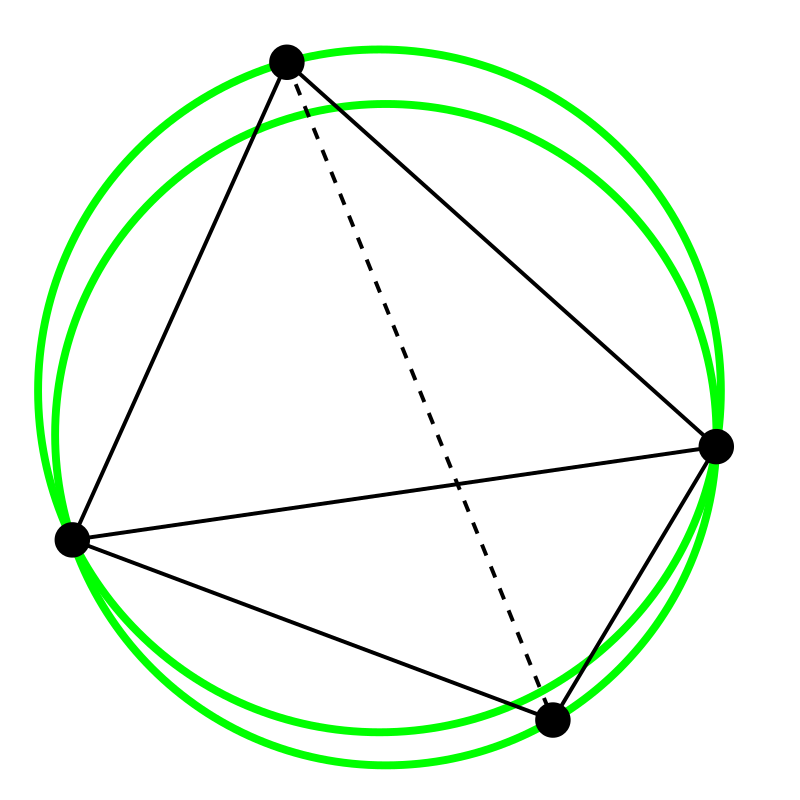
\includegraphics[width=8cm]{/Users/gabry/Desktop/Latex/Foto_Relazione_PCS/flip.jpg}
\end{center}

\item \textbf{Rimozione del \emph{Supertriangolo}}.  Il triangolo di partenza viene rimosso,  lasciando solo la triangolazione conclusiva.

\end{itemize}

    
\newpage
\section{Strutture C++}
Segue la descrizione della struttura in linguaggio C++ utilizzata per l'implementazione dell'algoritmo risolutivo.

\subsection{Struct Point e Triangle}
Ai fini della memorizzazione dei punti e dei triangoli,  sono state create due \emph{struct} C++,  una adibita alla costruzione di oggetti \textbf{Point} e una per gli oggetti \textbf{Triangle}.  \\

\begin{itemize}

\item  Struttura \textbf{Point}:
\begin{lstlisting}
struct Point
{
    double x, y;
    Point(double x = 0, double y = 0) : x(x), y(y){}
};
\end{lstlisting}
Il costruttore di questa struct inserisce negli attributi $_x$ e $_y$ i valori $x$ e $y$ che vengono passati in input.\\

\item Struttura \textbf{Triangle}:
\begin{lstlisting}
struct Triangle
{
    Triangle() = default;
    Triangle(const int& id, const Point& p1, const Point& p2, const Point& p3);

    int id;
    Point p1, p2, p3;
    array<double,3> angles;
    array<int,3> adjacentIds = {-1, -1 , -1};

    bool IsInTheCircle(const Point& d);
    bool IsInTheTriangle(const Point& d);
    unsigned int FindAdjacent(const int& id);
    friend ostream& operator << (ostream& os, const Triangle& t)
    {
        os << "Id: " << t.id
           << " (" << t.p1.x << ", " << t.p1.y << ")"
           << " (" << t.p2.x << ", " << t.p2.y << ")"
           << " (" << t.p3.x << ", " << t.p3.y << ")";
        return os;
    }
    friend class Triangulation;

};
\end{lstlisting}
Qui figurano attributi e metodi il cui scopo è esplicitato dal nome,  insieme all'override dell'operatore $<<$ per facilitare la visualizzazione degli oggetti \textbf{Triangle}.  Inoltre,  la classe \textbf{Triangulation} è dichiarata come \enquote{amica}.
\end{itemize}

\subsection{Class Triangulation}
All'interno di questa classe sono dichiarati i metodi che concorrono direttamente alla creazione della triangolazione.

\begin{lstlisting}
class Triangulation
{
private:
    vector<Triangle> triangles;

public:
    Triangulation() = default;
    Triangulation(const vector<Triangle>& triangles): triangles(triangles) {}

    list<int> Connect(const int& id, const Point& d);
    void Flip(const int& FirstId, const unsigned int& i,  
    const int& SecondId, const unsigned int& j);
    
    void Verify(list<int>& ids);
    vector<Triangle> Delaunator(vector<Point>& points);

    friend ostream& operator << (ostream& os, const Triangulation& tt)
    {
        for (const Triangle& t : tt.triangles)
            os << t << endl;
        return os;
    }
};
\end{lstlisting}
È inoltre dichiarato come attributo privato il vettore che conterrà gli oggetti \textbf{Triangle} che comporranno la triangolazione finale.
In aggiunta,  è eseguito l'override dell'operatore $<<$ al fine di stampare i triangoli della triangolazione e visualizzarla più agilmente. 
In particolare,  il metodo \enquote{Delaunator} è il responsabile della creazione della triangolazione,  il quale chiama gli altri metodi della classe.
\newpage
\subsection{Class Reader}
La classe \textbf{Reader} è adibita alla lettura del file testo o csv di input e all'estrazione del dataset di punti.

\begin{lstlisting}
class Reader
{
private:
    string input;
    string line;
    ifstream file;
    vector<Point> points;
public:
    Reader() = default;
    vector<Point> MakeVector(const string& input);
};
\end{lstlisting}

\subsection{Override di Operatori}
Al fine di eseguire agilmente le varie operazioni di confronto tra oggetti di tipo \textbf{Point}, \textbf{Triangle} e vettori di \textbf{Point} e vettori di \textbf{Triangle},  sono eseguiti i seguenti override degli operatori di differenza e uguaglianza tra gli oggetti sopra citati.  Sono inoltre create funzioni \enquote{inline} per il calcolo del prodotto scalare e esterno e della norma per oggetti \textbf{Point}.

\begin{lstlisting}
// override operatore di differenza fra oggetti Point
inline Point operator - (const Point& p1, const Point& p2)
{
    return Point(p1.x-p2.x,p1.y-p2.y);
}

// operatore prodotto scalare tra punti
inline double operator * (const Point& p1, const Point& p2)
{
    return p1.x*p2.x + p1.y*p2.y;
}

// operatore prodotto esterno
inline double prod(const Point& p1, const Point& p2)
{
    return p1.x*p2.y - p2.x*p1.y;
}

// operatore uguaglianza tra oggetti Point
inline bool operator == (const Point& p1, const Point& p2)
{
    return (p1.x==p2.x && p1.y==p2.y);
}

// operatore uguaglianza tra oggetti Triangle
inline bool operator == (const Triangle& t1, const Triangle& t2)
{
    return (
        (t1.p1 == t2.p1 && t1.p2 == t2.p2 && t1.p3 == t2.p3) ||
        (t1.p1 == t2.p1 && t1.p2 == t2.p3 && t1.p3 == t2.p2) ||
        (t1.p1 == t2.p2 && t1.p2 == t2.p1 && t1.p3 == t2.p3) ||
        (t1.p1 == t2.p2 && t1.p2 == t2.p3 && t1.p3 == t2.p1) ||
        (t1.p1 == t2.p3 && t1.p2 == t2.p1 && t1.p3 == t2.p2) ||
        (t1.p1 == t2.p3 && t1.p2 == t2.p2 && t1.p3 == t2.p1));
}

// creazione funzione inline NORMA per oggetto Point
inline double norm(const Point& p)
{
    return sqrt(p.x*p.x + p.y*p.y);
}

// operatore di uguaglianza tra vettori di oggetti Point
inline bool operator == (const vector<Point>& vec_p1, const vector<Point>& vec_p2)
{
    unsigned int n = vec_p1.size(); // se n = 0 considero gli oggetti uguali
    bool equal = true;

    for (unsigned int i = 0; i < n; i++)
    {
        if (!(vec_p1[i] == vec_p2[i]))
        {
            equal = false;
            break;
        }
    }
    return equal;
}
\end{lstlisting}
\newpage
\begin{lstlisting}
// operatore di uguaglianza vettori di triangoli
inline bool operator == (const vector<Triangle>& vec_t1, const vector<Triangle>& vec_t2)
{
    unsigned int n = vec_t1.size(); // se n = 0 considero gli oggetti uguali
    bool equal = true;

    for (unsigned int i = 0; i < n; i++)
    {
        if (!(vec_t1[i] == vec_t2[i]))
        {
            equal = false;
            break;
        }
    }
    return equal;
}
\end{lstlisting}

\section{Descrizione delle funzioni}
Di seguito è fatta una descrizione dettagliata della struttura delle funzioni che compongono l'algoritmo.

\subsection{Funzione MakeVector}\label{sez 4.1}
La prima funzione discussa è la funzione responsabile della memorizzazione del dataset all'interno del calcolatore.  Questa riceve in input una stringa contenente l'indirizzo del file e,  attraverso un ciclo \emph{while},  itera sulle righe del file inserendo tramite \emph{push\_back} l'oggetto \textbf{Point} nel vettore \textbf{points} cui ha accesso poiché attributo della classe di cui questo metodo è membro.
Dunque,  questa funzione ritorna un vettore di oggetti di tipo \textbf{Point}.

\begin{lstlisting}
vector<Point> Reader::MakeVector(const string& input)
{
    file.open(input);
    getline(file,line);
    while (!file.eof())
    {
        double id, x, y;
        getline(file,line);
        istringstream cast(line);

        cast >> id >> x >> y;
        points.push_back(Point(x,y));
    }
    file.close();
    return points;
}
\end{lstlisting}

\subsection{Funzione Delaunator}
La funzione \textbf{Delaunator} è la funzione principale dell'intero processo di triangolazione,  la quale chiama le altre funzioni della sua classe.  
Nel dettaglio,  questa riceve in input il vettore \textbf{points} creato dalla funzione descritta in \ref{sez 4.1}.  \textbf{Delaunator} controlla che non vi siano ripetizioni nel dataset e,  in caso,  le elimina attraverso la funzione \textbf{Repetitions}
\begin{lstlisting}
vector<Point> Repetitions(vector<Point>& vecp)
{
    for (unsigned int i = 0; i < vecp.size(); i++)
    {
        for (unsigned int j = 0; j < vecp.size(); j++)
        {
            if (j != i)
            {
                if (vecp[j] == vecp[i])
                {
                    vecp.erase(vecp.begin()+j);
                }
            }
        }
    }
    return vecp;
}
\end{lstlisting}
Dopodiché,  procede al calcolo dei vertici del \emph{Supertriangolo} iterando sui punti contenuti in \textbf{points} alla ricerca di massimo e minimo delle coordinate.
In seguito,  per ogni punto nel dataset,  per pgni triangolo della triangolazione corrente,  controlla che tale punto sia all'interno del suo circocerchio attraverso il metodo \textbf{IsInTheCircle} e che tale punto sia all'interno del triangolo stesso attraverso il metodo \textbf{IsInTheTriangle}: in caso di condizione verificata per entrambe le funzioni,  il punto non è da considerarsi valido ai fini della triangolazione e viene pertanto unito ai vertici del triangolo corrente.  Immediatamente dopo è chiamata la funzione \textbf{Verify} in cui sono eseguiti i controlli della condizione di Delaunay e l'operazione di Flip, se necessario.

\noindent Infine,  si procede alla rimozione dei bordi appartenenti al \emph{Supertriangolo} di partenza.

\noindent La funzione ritorna il vettore contenente la triangolazione finale.

\begin{lstlisting}

vector<Triangle> Triangulation::Delaunator(vector<Point>& points) // delaunator
{
    vector<Point> points_norep = Repetitions(points);
    unsigned int n = points.size();
    triangles.reserve(2*n); //allocazione preventiv di memoria

    // define super triangle
    double minX, minY, maxX, maxY;
    minX = points_norep[0].x;
    minY = points_norep[0].y;
    maxX = minX;
    maxY = minY;

    for (unsigned int i = 1; i < n; i++)
    {
        minX = min(minX, points_norep[i].x);
        minY = min(minY, points_norep[i].y);
        maxX = max(maxX, points_norep[i].x);
        maxY = max(maxY, points_norep[i].y);
    }

    // width e height della scatola che racchiude i punti
    double dx, dy, midX;
    dx = maxX - minX;
    dy = maxY - minY;
    midX = (maxX + minX) / 2;

    // punti scelti fuori dal dataset in modo tale da assicurare che il super triangolo contenga tutti i punti
    Point p1(minX - 2 * dx, minY - dy / 2);
    Point p2(maxX + 2 * dx, minY - dy / 2);
    Point p3(midX, 2 * maxY + dy);
   
    triangles.push_back(Triangle(0, p1, p2, p3));
    list<int> newIds;

    for (const Point& p : points_norep)
    {
        int n = triangles.size();
        for (int id = 0; id < n; id++)
        {
            Triangle t = triangles[id];
            if (t.IsInTheCircle(p))
            {
                if (t.IsInTheTriangle(p))
                {
                    newIds = Connect(id, p);
                    Verify(newIds); // qui viene chiamata la funzione di Flip()
                    break;
                }
            }
        }

    }
\end{lstlisting}
\newpage
\begin{lstlisting}
    //rimozione super triangle iniziale
    triangles.erase(remove_if(triangles.begin(), triangles.end(),
                              [&](Triangle& t)
                              {
                                  return t.p1 == p1 ||
                                         t.p1 == p2 ||
                                         t.p1 == p3 ||
                                         t.p2 == p1 ||
                                         t.p2 == p2 ||
                                         t.p2 == p3 ||
                                         t.p3 == p1 ||
                                         t.p3 == p2 ||
                                         t.p3 == p3;

                              }), triangles.end());

    return triangles;
}
\end{lstlisting}

\subsection{Funzioni di controllo sui punti}
In questa sezione sono elencati i metodi più semplici di controllo sui punti.

\begin{itemize}
\item \textbf{isCounter}.  Riceve in punt tre oggetti \textbf{Point} e verifica che il prodotto esterno tra il lato numero uno e il lato numero tre sia $\geq 0$.
\begin{lstlisting}
bool isCounter(const Point& p1, const Point& p2, const Point& p3)
{
    double s;
    s = prod(p2-p1, p3-p1);
    return (s >= 0);
}
\end{lstlisting}
\item \textbf{IsInTheCircle} e \textbf{IsInTheTriangle}.  Provenienti entrambi dalla classe \textbf{Triangle},  questi metodi ricevono in input un oggetto \textbf{Point} e controllano che questo cada,  rispettivamente, nel circocerchio del triangolo su cui questa funzione viene chiamata e nel triangolo stesso.
\begin{lstlisting}
bool Triangle::IsInTheCircle(const Point& d)
{
    Matrix<double, 3, 3> mat;
    mat << p1.x-d.x, p1.y-d.y, (p1.x-d.x)*(p1.x-d.x) + (p1.y-d.y)*(p1.y-d.y),
        p2.x-d.x, p2.y-d.y, (p2.x-d.x)*(p2.x-d.x) + (p2.y-d.y)*(p2.y-d.y),
        p3.x-d.x, p3.y-d.y, (p3.x-d.x)*(p3.x-d.x) + (p3.y-d.y)*(p3.y-d.y);

    return (mat.determinant() > 0);
}

bool Triangle::IsInTheTriangle(const Point& d)
{
    return (isCounter(p1, p2, d) && isCounter(p2, p3, d) && isCounter(p3, p1, d));
}
\end{lstlisting}
\item \textbf{FindAdjacent}.  Il metodo è chiamato su un triangolo della triangolazione.  Prende in input l'Id di un triangolo e ritorna l'indice del lato di adiacenza?
\end{itemize}


\subsection{Costruttore Triangle e metodi della classe Triangulation}
Il costruttore \textbf{Triangle},  oltre a creare l'oggetto il cui nome fa riferimento,  si occupa anche di calcolare gli angoli interni di tale triangolo.
\begin{lstlisting}
Triangle::Triangle(const int& id, const Point& p1, const Point& p2, 
const Point& p3):
    id(id), p1(p1), p2(p2), p3(p3)
{
    
    angles[0] = acos((p2-p1)*(p3-p1)/(norm(p2-p1)*norm(p3-p1)));
    angles[1] = acos((p3-p2)*(p1-p2)/(norm(p3-p2)*norm(p1-p2)));
    angles[2] = acos((p1-p3)*(p2-p3)/(norm(p1-p3)*norm(p2-p3)));
}
\end{lstlisting}

Per quanto riguarda i metodi della classe \textbf{Triangolazione}:

\begin{itemize}
\item \textbf{Connect}. Il metodo \textbf{Connect} viene chiamato all'interno di \textbf{Delaunator} una volta che un punto viene localizzato all'interno di un triangolo.  La funzione connette il punto ai vertici del triangolo corrente,  creando tre nuovi triangoli.  A questi vengono assegnati gli Id nel segunte modo: il primo triangolo creato riceve l'Id del triangolo di partenza, il secondo e il terzo ricevono degli Id nuovi all'interno della triangolazione. In seguito, vengono aggiornate le adiacenze per i nuovi triangoli e per i triangoli adiacenti al triangolo di partenza.  Il metodo restituisce gli Id dei triangoli creati sotto forma di lista.

\item \textbf{Verify}. Il metodo \textbf{Verify} viene chiamato da \textbf{Delaunator} subito dopo \textbf{Connect}.  Riceve in input la lista degli Id dei triangoli dei quali si vuole effettuare la verifica dell'ipotesi di Delaunay.  Il metodo accede sequenzialmente agli elementi della lista.  Ad ogni triangolo si valuta, per ogni triangolo adiacente (con un ciclo for che effettua al più 3 iterazioni),  se gli angoli opposti al lato di adiacenza sommino a più di 180°.  Se ciò accade, viene chiamato il metodo \textbf{Flip} e viene aggiunto alla lista il triangolo adiacente in questione. Avendo modificato il triangolo, ripetiamo il controllo su di esso, finchè non è più necessaria alcuna operazione di Flip. A quel punto eliminiamo il primo elemeto della lista, e procediamo con il successivo, finchè essa non è vuota.

\item \textbf{Flip}. Il metodo \textbf{Flip} riceve in input gli Id dei triangoli di cui fare il Flip e gli indici sul triangolo del lato di adiacenza.  Il metodo crea i due flippati, a cui assegna gli stessi Id in input.  In seguito vengono aggiornate le adiacenze sui nuovi triangoli e sui triangoli ad essi adiacenti.

\end{itemize}

\section{Test}
Sono progettati ed eseguiti test per assicurarsi che ogni funzione svolga correttamente il compito per cui è stata progettata.  I test sono raggruppati,  a rigor di logica,  in quattro sezioni:
\begin{itemize}
	\item \textbf{Operators\_test}.  Raggruppa i test in merito alle operazioni di override degli operatori di uguaglianza e differenza tra oggetti della classe \textbf{Point} e \textbf{Triangle}.  Inoltre,  vengono testate delle funzioni definite attraverso il comando \emph{inline} che calcolano il prodotto scalare,  il prodotto esterno e la norma per oggetti di tipo \textbf{Point}.  
	\item \textbf{Reader\_test}.  Contiene i test sui due metodi facenti parte della classe Reader: \emph{MakeVector} e \emph{Repetitions}. Entrambi i test si occupano di verificare la correttezza del loro funzionamento.
	\item \textbf{Triangulation\_test}.  All'interno di questo file sono raggruppati i testi in merito alle funzioni che si occupano di operazioni sui triangoli e,   nello specifico,  della triangolazione vera e propria.
\end{itemize}

\section{Costo computazionale}
L'algoritmo di triangolazione descritto e implementato è largamente utilizzato in applicazioni reali,  come analisi F.E.M.  e applicazioni artistiche varie.  Inoltre,  il suo costo computazionale,  pur variando sulla base del numero di punti presi in input,  è dell'ordine di $\Omega(n\cdot \log n)$.  Questo può essere scomposto in due parti:

\begin{itemize}
	\item[1.] La costruzione del Supertriangolo iniziale prevede un numero di operazioni proporzionale a $\Omega(n)$ in quanto occorre trovare il minimo e il massimo valore delle coordinate dei punti attraverso una ricerca esaustiva.
	\item[2.] L'inserimento sequenziale del punti viene ripetuto $n$ volte e per ogni punto viene applicato  l'algoritmo di Bowyer\-Watson che ha complessità $\Omega( \log n)$.
\end{itemize}
In conclusione,  l'algoritmo ha costo computazionale dell'ordine di $\Omega(n\cdot \log n)$.
\end{document}


